% starting the actual presentation for Wednesday 
\documentclass{beamer}
\usetheme{Warsaw}

% title page details 
\title{Bayesian Inference for Gaussian Graphical Models}
\author{Anthony Bernardi\inst{1} , Aidan Elias\inst{1}} 
\institute{\inst{1} University of Kentucky - Department of Statistics} 
\date{\today}

\begin{document}

% title page as the first slide 
\begin{frame}
   \titlepage 
\end{frame}

% table of contents 
\begin{frame}{Overview} 
  \tableofcontents
\end{frame} 

% establishing the structure 
\section{Introduction}
\section{Literature Review}
\section{Data and Methodology}
\section{Results and Future Directions}
\section*{References}

% getting into introduction
\begin{frame}{Introduction}
  
  \begin{itemize}
    \item Introduction and Data Familiarity
    \item Gibbs Sampling Technique and Prior Choice 
    \item Graph and Inference
    \item Precision Matrix Inference 
  \end{itemize}

\end{frame}

% lit review 
\begin{frame}{Literature Review}

  \begin{itemize}
    \item Papers of Note for this Study 
      \begin{itemize}
        \item \textit{Bayesian Inference for the Multivariate Normal} Penny, 2014 
        \item \textit{Bayesian Variable Selection in Linear Regression} Mitchell and Beauchamp 1988   
        \item \textit{Variable Selection Using Shrinkage Priors} Li and Pati 2017
        \item \textit{Sparsity Information and Regularization in the horseshoe and other shrinkage priors} Piironen and Vehtari 2017
      \end{itemize}
  \end{itemize}
\end{frame}

\begin{frame}{Data and Methodology}

  \begin{itemize}
    \item Data Cleaning and Feature Engineering:
      \begin{itemize}
        \item Provided dataset isolated to include only proteins for precision matrix inference  
      \end{itemize}
    \item Prior Specification and Full Conditionals: 
      \begin{itemize}
        \item Wishart Prior for Precision Matrix 
        \item Regularized Horseshoe Prior for Regression Coefficients used over Spike and Slab
      \end{itemize}
    \item Gibbs Sampling: 
      \begin{itemize}
        \item Full Conditionals for Precision Matrix and Regression Coefficients
        \item Gibbs Sampling done in the canonical parameterization 
      \end{itemize}
  \end{itemize}
\end{frame}

% results and future directions 
\begin{frame}{Results and Future Directions}
  \begin{itemize}
    \item Results: 
      \begin{itemize}
        \item Posterior Inference for Precision Matrix 
        \item Posterior Inference for Regression Coefficients 
      \end{itemize}
    \item Future Directions: 
      \begin{itemize}
        \item Further exploration of the regularized horseshoe prior 
        \item Application to other datasets 
      \end{itemize}
  \end{itemize}
\end{frame}

% some proposed graphical results 
\begin{frame}{Proposed Graphical Results - Phase 1}
\centering
    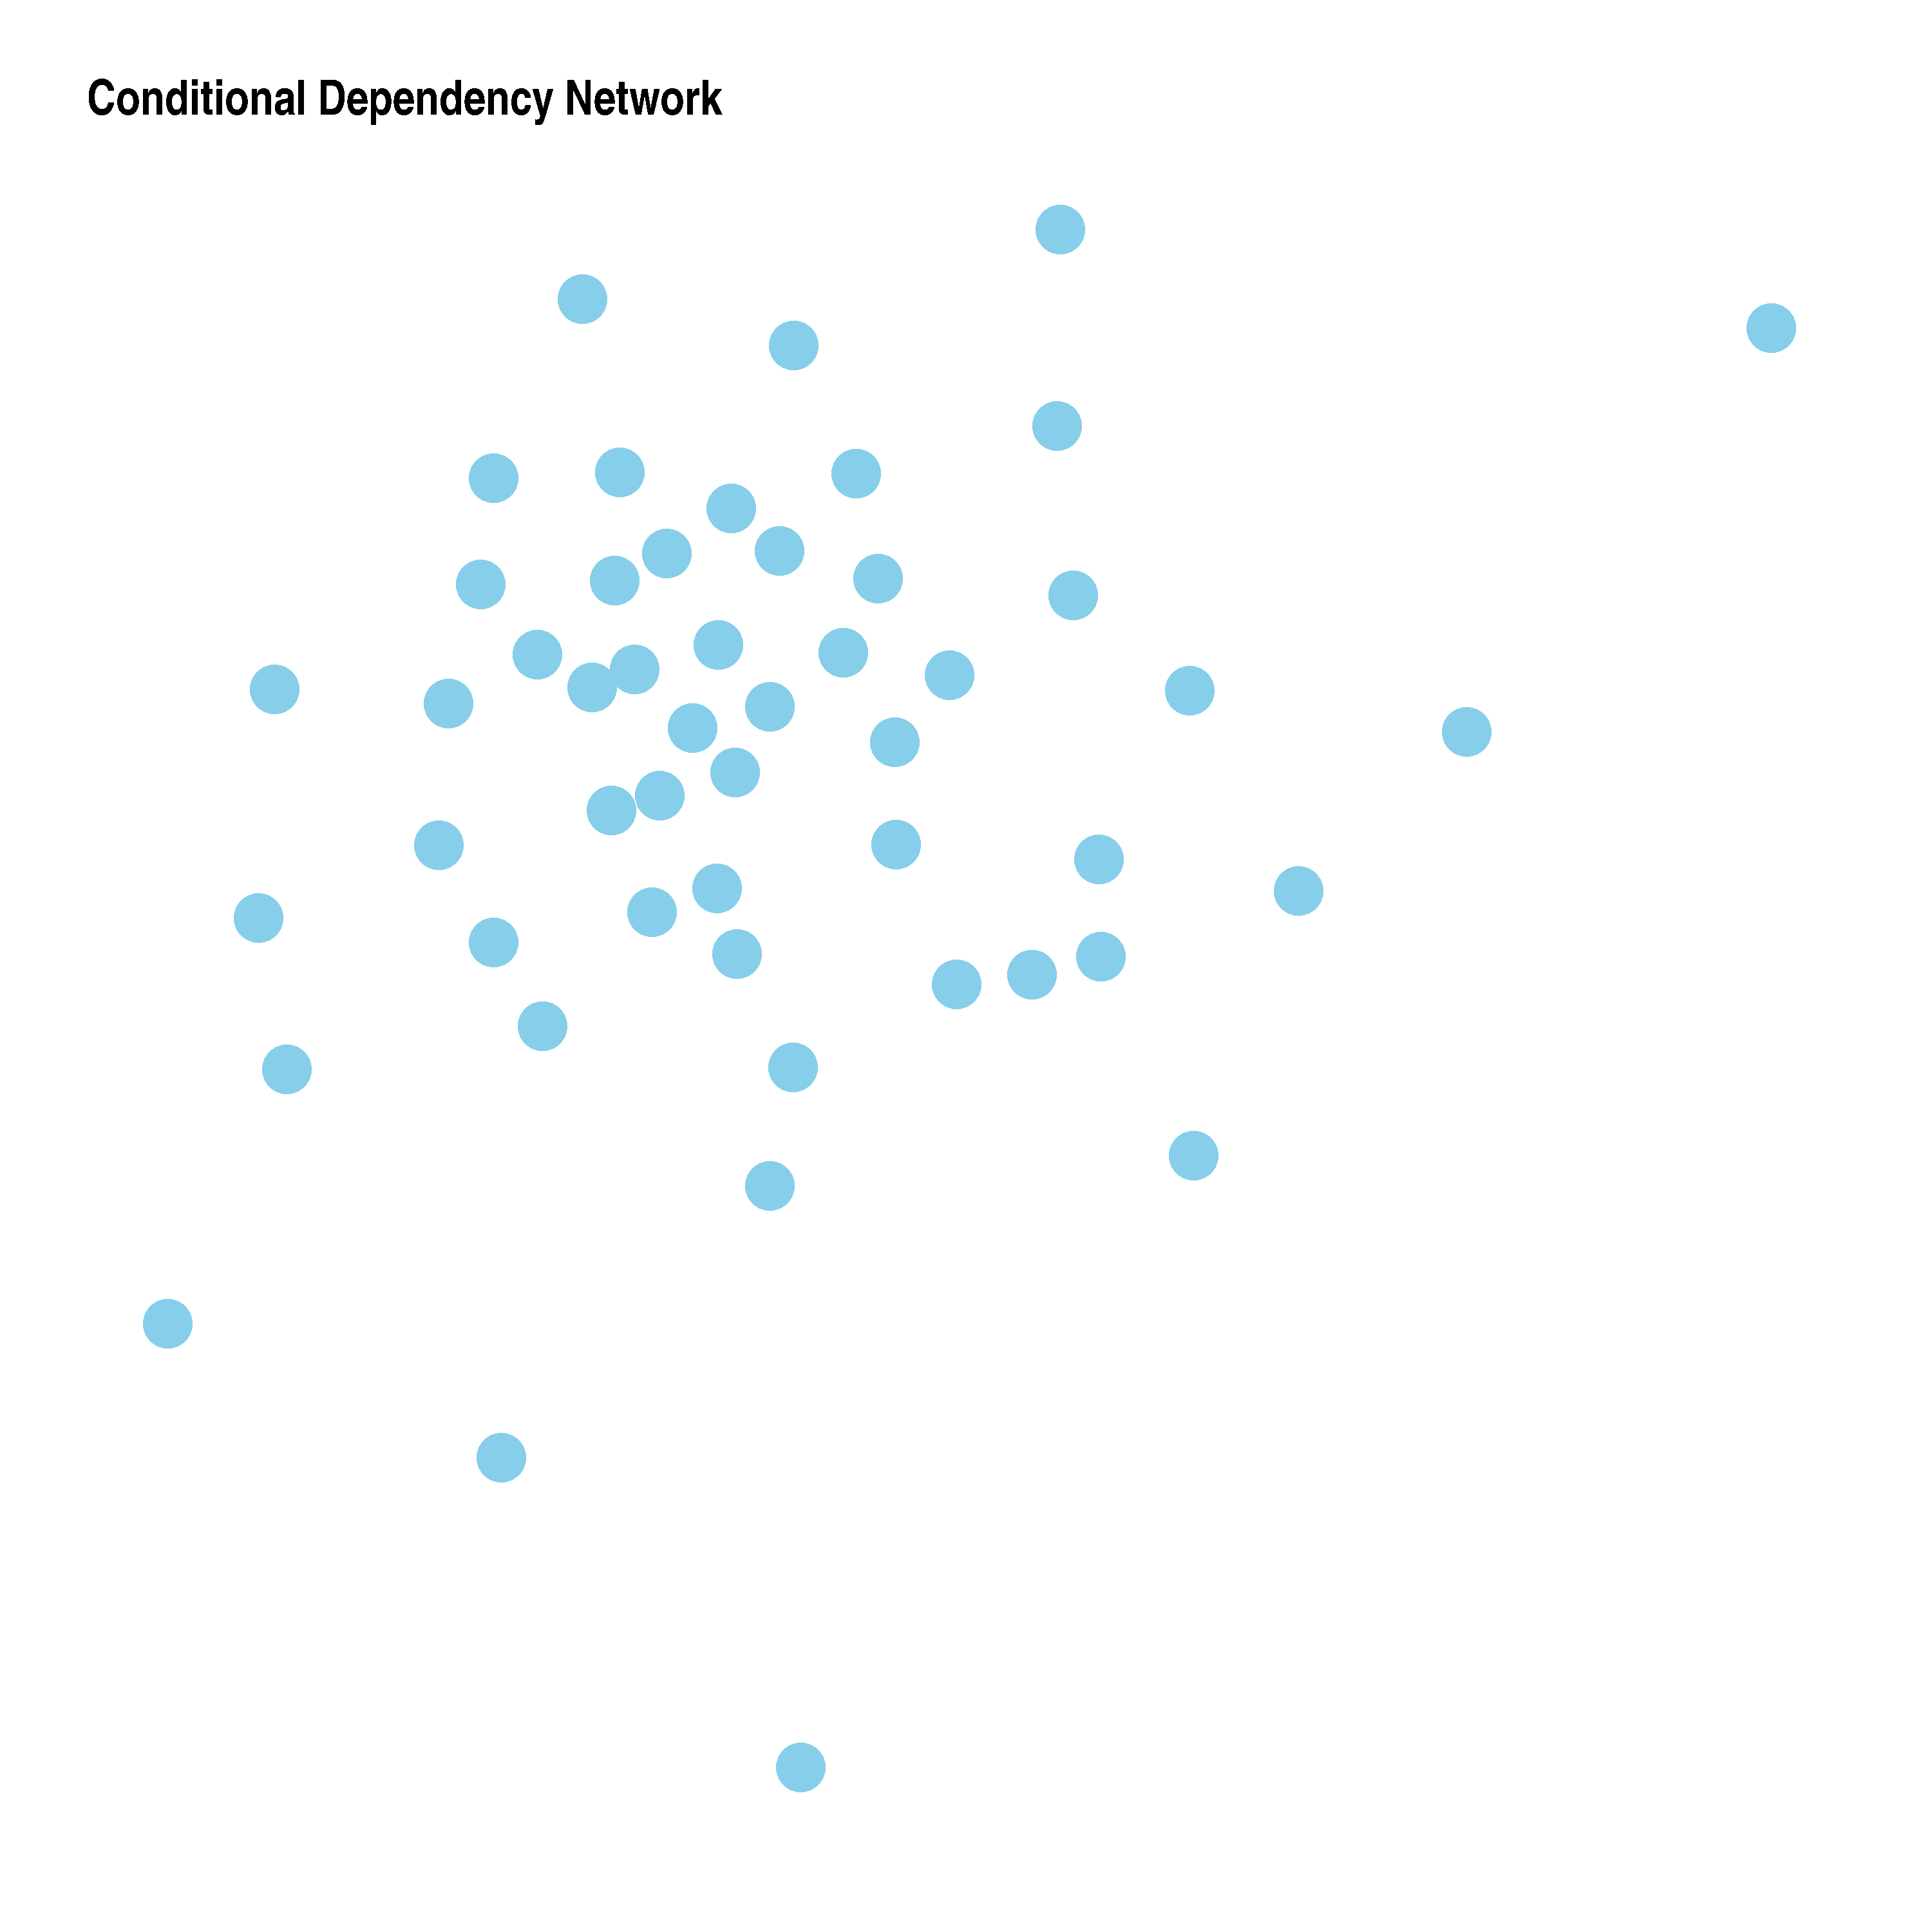
\includegraphics[scale=0.33]{Conditional_density_network.png}
\end{frame}

% option 2
\begin{frame}{Proposed Graphical Results - Phase 2}
\centering
    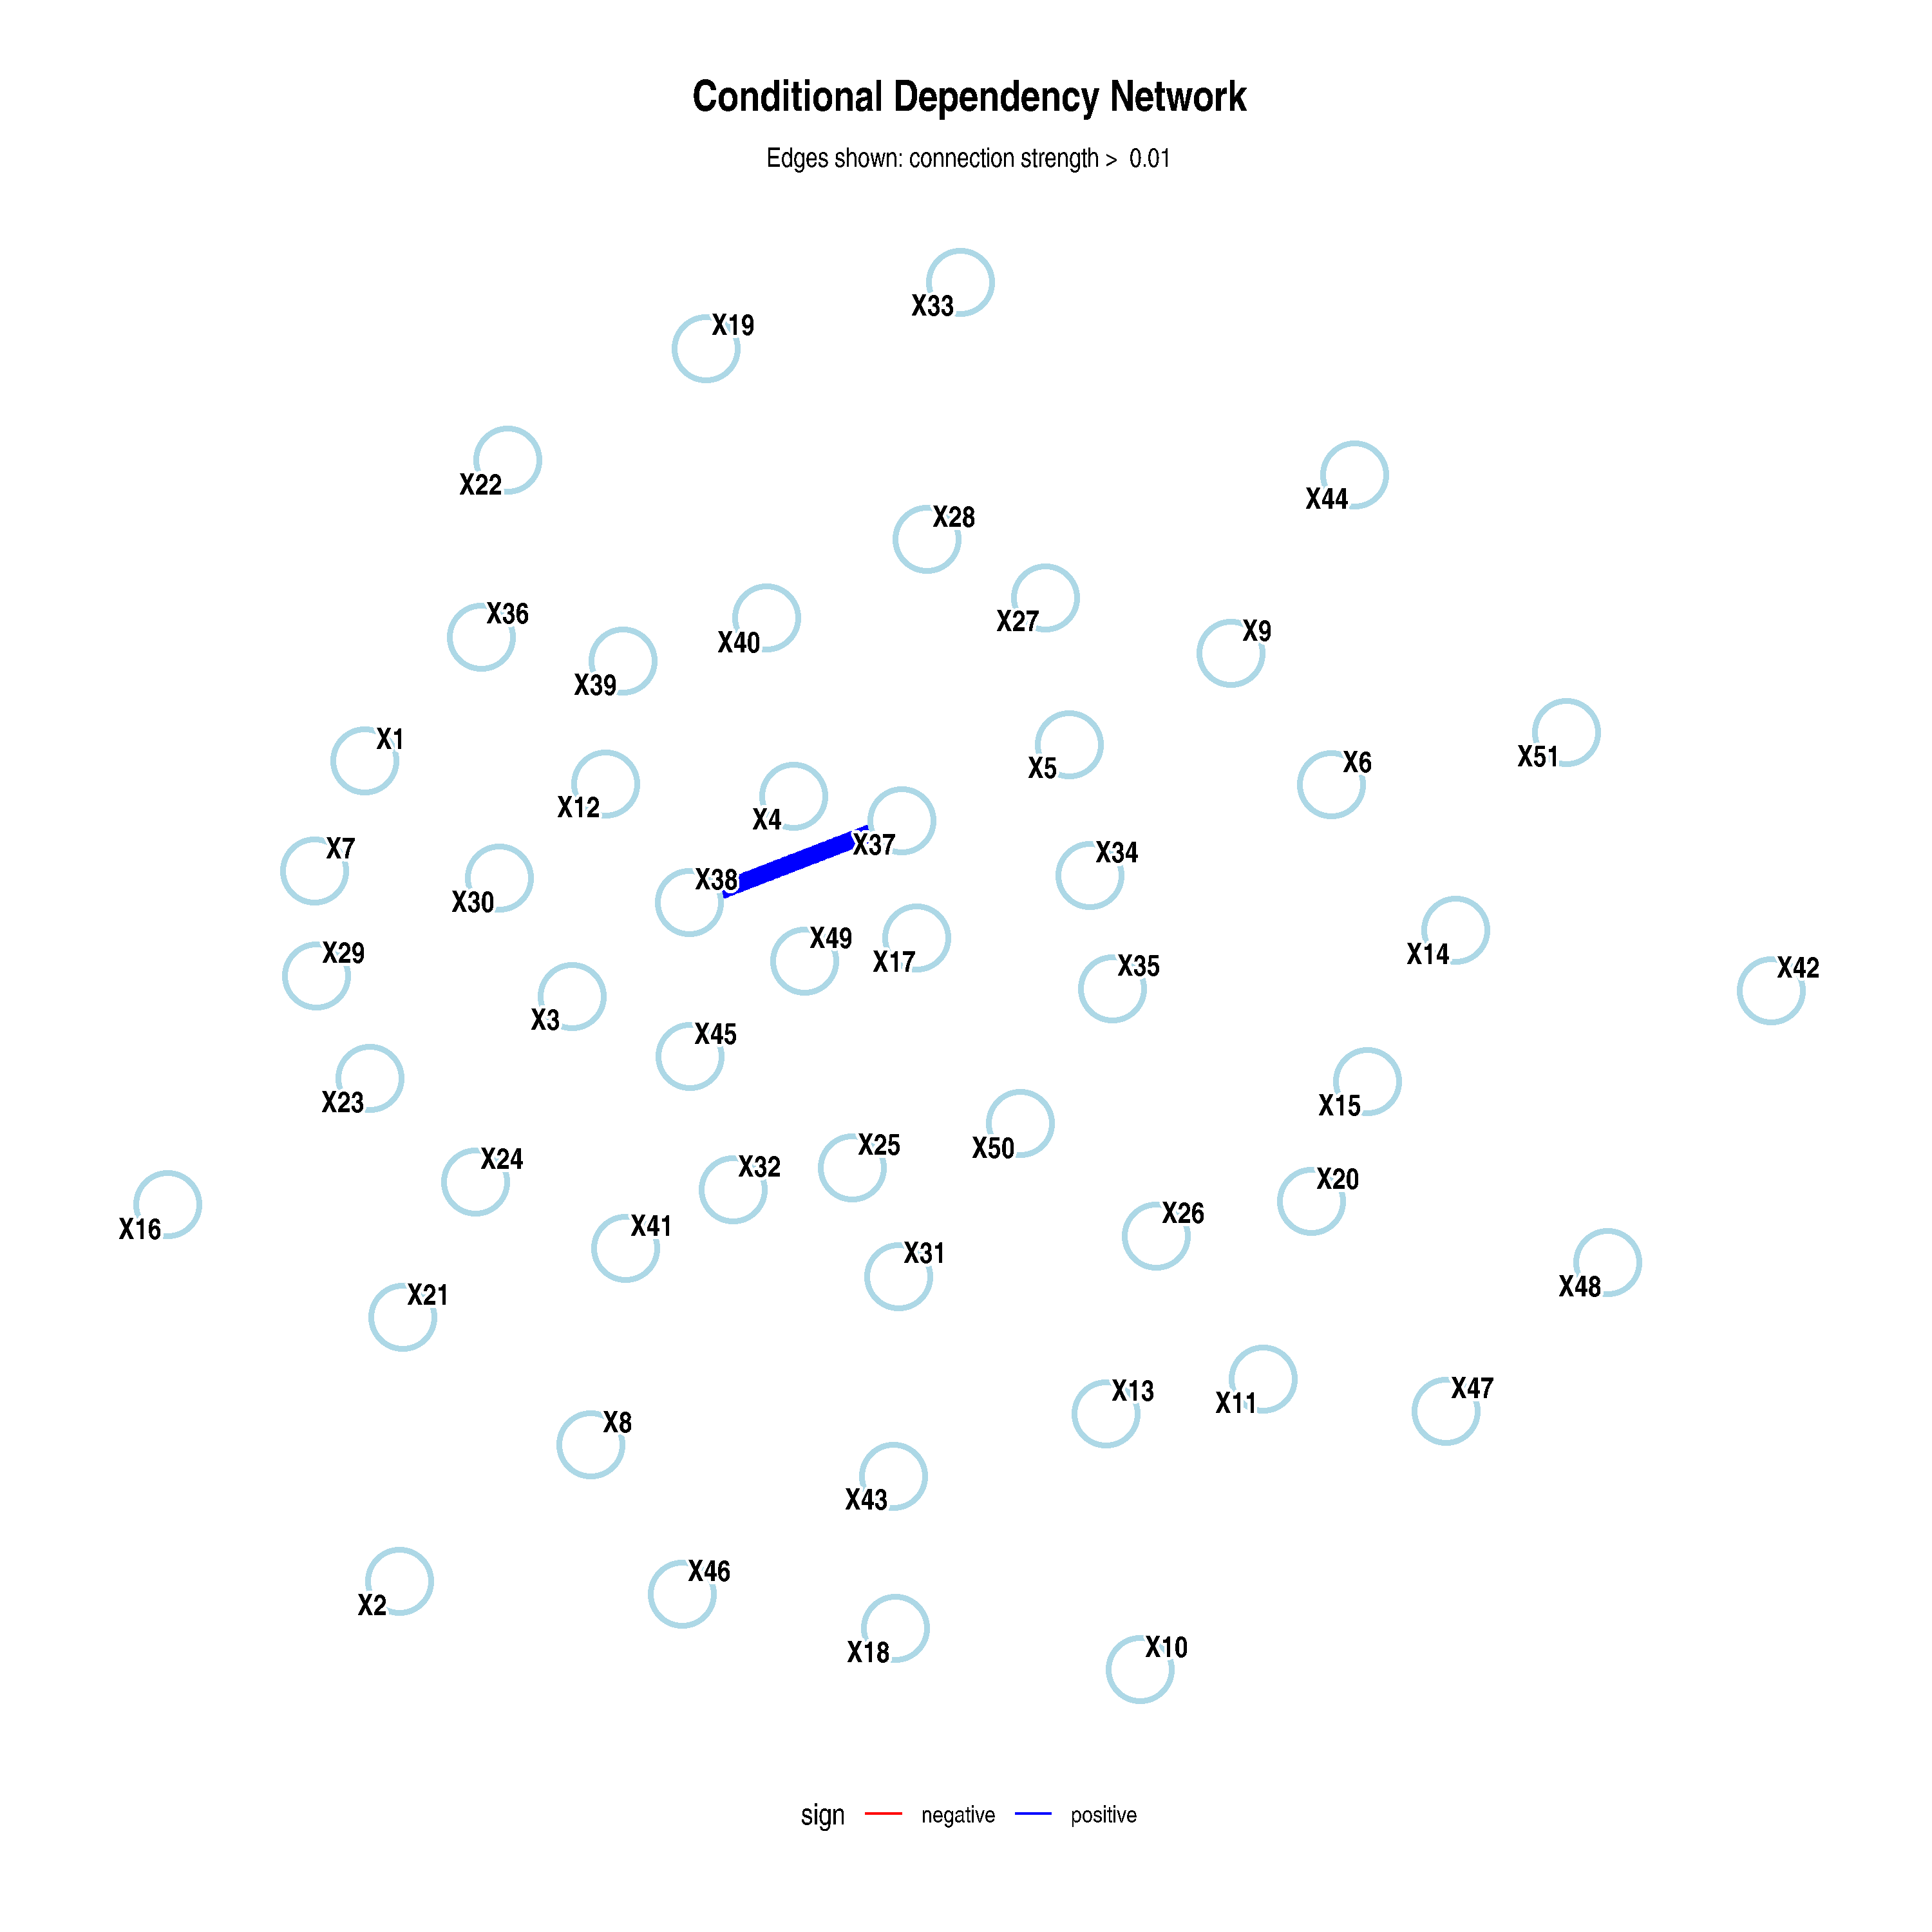
\includegraphics[scale=0.25]{Conditional_density_network_labeled.png}
\end{frame}

% future directions 
\begin{frame}{Future Directions}
    \begin{itemize}
        \item Evaluation of Prior Choice Over Alternative
        \item More analysis of Protein Network
        \item Further diagnosis of Gibbs sampler 
    \end{itemize}
\end{frame}






















\end{document}
